\documentclass[a4paper,12pt]{article}
\usepackage{graphicx}
\usepackage{hyperref}   % use for hypertext links, including those to external documents and URLs

\begin{document}



\begin{center}
\begin{Huge}
\textbf{{\LARGE Group Report\\ Unit Test Visualisation }}
\linebreak
\linebreak
\linebreak
\linebreak
\end{Huge}\end{center}




\begin{small}
\begin{flushleft}
\textbf{Team:} Group 4
\\
\textbf{Course:} ELEN7046 - Software Technologies and Techniques
\\
\textbf{Date Submitted:} 25 June 2012
\\
\textbf{Source \& Documentation:} https://github.com/KeaganPhillips/Wit-Group-4-project
\linebreak
\linebreak
\linebreak
\linebreak
\linebreak
\end{flushleft}
\end{small}


\begin{flushleft}
\textbf{{\large Abstract}}
\end{flushleft}
The design and implementation of a software visualisation tool for unit testing is presented. The visualisation tool is to be used to graphically display, enhance and ... unit tests. The development of both the unit tests and its visualisation are discussed. The tool was implemented using TDD and uses C\# Reflection to obtain the necessary information which was then sent to the visualiser to display. The implementation suggests that the tool can play an important role in software visualistaion education.    
\clearpage


\tableofcontents


\clearpage

\section{Introduction}
This paper presents a report of an application that links software visualisation and software education. In the literature, it is stipulated that software visualization encompasses the development and evaluation of methods for graphically representing different aspects of software, including its structure, its execution, and its evolution.\\
\linebreak  
The aspect of software that we present in this report is Unit Testing\cite{unitTests}. The primary goal of unit testing is to take the smallest piece of testable software in the application, isolate it from the remainder of the code, and determine whether it behaves exactly as expected. Each unit is tested separately before integrating them into modules to test the interfaces between modules.
This testing mode is a component of Extreme Programming (XP)\cite{xp}, a pragmatic method of software development that takes a precise approach to building a product by means of continual testing and revision.\\
\linebreak  
Unit testing involves only those characteristics that are vital to the performance of the unit under test. This encourages developers to modify the source code without immediate concerns about how such changes might affect the functioning of other units or the program as a whole. Once all of the units in a program have been found to be working in the most efficient and error-free manner possible, larger components of the program can be evaluated by means of integration testing.\\
\linebreak  
In this report, we primarily demonstrate an application that visualises all the unit tests in a given program. The application discussed in this report visualises not only the unit tests, but also the class diagrams together with their public methods and properties.\\
\linebreak  
The remainder of this report is as follows. Section 2 discusses the licenses used in the development of the application. We provide the problem description in section 3, and discuss the approach we took to solve the problem in section 4. Installation process for the application is discussed in section 5. We provide a discussion on how the approach to the solution was implemented in section 6. In section 7, we discuss an analysis of our solution, and provide future works in section 8. We end the report with a conclusion


\section{License Agreement}
\subsection{Overview}
An analysis of software licenses was done considering the combination of both original work and third party components. The new BSD license also known as the 3-Clause BSD\cite{bds} license was chosen. The software and source code are made available under this license. Use, modification and redistribution is not restricted. 
\subsection{Components used and their license agreements}
The following lists the components used within the system together with their respective license agreements.
\begin{itemize}
\item \textbf{Coffee Script}: MIT license\cite{mit}
\item \textbf{Java script:} GNU GPL\cite{gnugpl}
\item \textbf{JQuery:} GNU GPL\cite{gnugpl}
\item \textbf{Kinetic.js:} GNU GPL\cite{gnugpl}
\item \textbf{PDF reporting tool:} CPOL\cite{cpol}
\item \textbf{ITextSharp:} GNU GPL\cite{gnugpl}
\end{itemize}

For the complete reference, please refer to the document 'ELEN7046 - Group4 - Licence Agreement.pdf'\cite{licenceDoc}

\section{Problem Description}
\subsection{Overview}
As good software practitioners, we always aspire to adopt the current best practices in our industry. In recent years the so called 'Agile' methodologies has become very popular with TDD\cite{tdd} (Test Driven Development) begin a very widely adopted agile practice. Today it is almost expected of developers to not only write program code, but also create automated unit tests and apply other TDD practices.
\subsection{Problems with respect to Unit Tests}
Writing automated unit tests comes with its own unique problems. Our project attempts to address some of these shortcomings by proposing a framework against which developers can write their automated tests. The end result should give developers a broad and high level view of all unit tests, making it easier for them to get a holistic view of all the unit tests in the system under test.
\subsubsection{Large Complex projects}
Tests can become difficult to read and understand especially as the suite of tests rapidly grows in number and complexity with each build deployed. It is very easy for a developer to get lost in the detail by reading the actual automated test code. This is because the developer can only view one automated unit test at a time, making it difficult to see the whole picture. 
\subsubsection{Comments in tests}
Many developers don't write adequate comments in their tests leaving other team members in the dark with regard to what their initial intent was.\\
\linebreak
It's never good to have a test or group of tests that isn't well understood (even though the test(s) may pass). Tests are only useful when the context of the tests is clear and well understood.  
\subsubsection{The Learning Curve}
The above described scenarios make it difficult for the development team to evolve a system over time. The result being that the learning curve is often very steep for new developers joining the development team as well as for junior developers on the team.
\subsection{Proposed Solution}
What is needed is a framework that provides a convention that developers can follow where tests are written in a uniformed way. The system must provide a mechanism to visually display all tests without the developer having to zoom into the code to look at tests one at a time.\\
\linebreak
This, we believe should add tremendous value with respect to the learning of an existing and evolving code base.


\section{Approach}
Given the above stated requirement, the team proposed the following solution. A web application will be developed that provides a visual representation of the unit tests of the system under development

\subsection{High level design overview}
Figure \ref{fig1} depicts a high level overview of the proposed solution. This section will briefly discuss the key components of the system from right to left.

\begin{center}
	\begin{figure}
		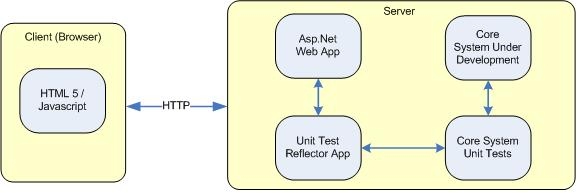
\includegraphics{system_overview.JPG}
			\caption{}
			\label{fig1}    
	\end{figure}	
\end{center}

\subsubsection{Core System Under Development}
This component represents the actual core application. This is the system that will actually run in the production environment and the application against which the unit tests will run. This system is completely oblivious of the other components depicted. Obviously developers must use an "interface driven" approach upon developing this component to facilitate modularity and enable for easy unit testing. The actual functional requirements for this application is beyond the scope of the project.\\
\linebreak
Please see section 3.1 of Keagan Phillips's individual report\cite{reportKeagan} for more a more in depth discussion regarding this component. 

\subsubsection{Core System Unit Tests}
This component represents the actual unit test project and contains automated unit tests. These tests target the "Core System Under Development" component.\\
\linebreak  
Tests must be written following a predefined convention\cite{UTconvention}. The development team used the TDD\cite{tdd} (Test Driven Development) technique and "Given / When / Then"\cite{gwt} convention for specifying tests scenarios.\\
\linebreak  
Please refer to section 3.2 of Keagan Phillips's individual report\cite{reportKeagan} for more detail on this component.\\
\linebreak  
Please see the "Unit Test coding convention" document for an in depth discussion on how to wire automated tests using the provided framework.\cite{UTconvention}

\subsubsection{Unit Test Reflector}
This component's responsibility is to extract the unit test metadata embedded in the "Core System Unit Tests" component and transform that data into a C\# data structure. The team made use of the Microsoft Dot Net Framework's Reflection\cite{reflection} feature to achieve this goal. This data can then be collated and presented to the user in almost any format including document format (i.e. HTML page or PDF) or in our case visually and in pdf format as shown later on.\\
\linebreak  
Please refer to section 3.3 of Keagan Phillips's individual report\cite{reportKeagan} for more detail on this component.\\ 

\subsubsection{Asp.Net Web Application}
This component acts as a shell to host our solution in a web based environment. It calls the component 'Unit Test Reflector Application' upon receiving a web request. It then retrieves a data structure with the relevant test metadata. The data is then converted from a dot Net C\# object, to a JSON\cite{json} data structure to be transmitted back to the browser as an HTTP response.\\
\linebreak  
See Borelli’s report for more information.\cite{boreli}

\section{Installation Procedure}
blah.. blah...


\clearpage
\begin{thebibliography}{5}
\bibitem{unitTests} \url{http://www.extremeprogramming.org/rules/unittests.html}
\bibitem{xp} \url{http://www.extremeprogramming.org/}
\bibitem{bds} \url{http://www.opensource.org/licenses/BSD-3-Clause}
\bibitem{licenceDoc}  \begin{flushleft}
For the Group Project License Agreement see: 
\end{flushleft} \url{https://github.com/KeaganPhillips/Wit-Group-4-project/tree/master/Documentation/}
\bibitem{mit} \url{http://www.opensource.org/licenses/mit-license.html}
\bibitem{gnugpl} \url{http://www.gnu.org/copyleft/gpl.html}
\bibitem{cpol} \url{http://www.codeproject.com/info/cpol10.aspx}
\bibitem{tdd} \url{http://www.agiledata.org/essays/tdd.html}
\bibitem{reportKeagan} \begin{flushleft}
For Keagan Phillips's Individual Report see: 
\end{flushleft}\url{https://github.com/KeaganPhillips/Wit-Group-4-project/blob/8fe27d49f80fb3be2ed421e3bf7ce8daff002794/Documentation/Individual%20Reports/Individual%20Report%20-%20Keagan%20Phillips.pdf?raw=true}

\bibitem{UTconvention} \begin{flushleft}
For the Unit Test Coding Convention see:
\end{flushleft} \url{https://github.com/KeaganPhillips/Wit-Group-4-project/tree/master/Documentation/}

\bibitem{gwt} \begin{flushleft}
Structuring your test using Given/When/Then
\end{flushleft} \url{http://testedobjects.sourceforge.net/m2-site/main/documentation/docbkx/html/user-guide/ch03s04.html}

\bibitem{reflection} \url{http://msdn.microsoft.com/en-us/library/ms173183%28v=vs.80%29.aspx}


\bibitem{json} \begin{flushleft}
JSON (JavaScript Object Notation)
\end{flushleft} \url{http://www.json.org/}

\bibitem{boreli} \begin{flushleft}
For Boreli's Individual Report see:   
\end{flushleft} \url{https://github.com/KeaganPhillips/Wit-Group-4-project/tree/master/Documentation/}


\end{thebibliography}


\end{document}